\section{Rationale}
The proposed product is an acoustic panel primarily manufactured from recycled denim waste. According to \cite{EnvironmentalSustainabilityFashion}, the purpose of acoustic panels is to absorb sound waves to reduce noise and improve sound quality in different environments such as concerts and theatres. The primary end-of-life material being utilised for manufacturing these acoustic panels is post-consumer denim. Periyasamy and Periyasami \cite{CriticalReviewSustainability} identified that approximately 2.16 million tons of denim waste are abundant annually. By employing a fraction of the annual denim waste, the product not only provides a solution to textile waste but also provides a viable replacement substitution for traditional acoustic materials. \\ 
 
Manufacturing acoustic panels from recycled denim provides numerous benefits but have a focus on environmental sustainability. As previously mentioned, denim is responsible for 2.16 million tons of waste material, by repurposing the denim waste to manufacture the panels it helps divert textile waste from landfills, reducing the environmental impact associated with denim production and disposal. By replacing the traditional materials for acoustic panels with repurposed denim, the need for non-degradable synthetic fibres is significantly reduced \cite{burattiSustainablePanelsRecycled2016}. By providing a non-toxic, recycled product the acoustic panels contribute to a healthier indoor environment \cite{UltraTouchRecycledDenimb}. \\ 

This product's uniqueness stems from using recycled denim as the main material for acoustic panels, providing a sustainable and efficient substitute for traditional soundproofing options. Unlike conventional fabrics, recycled denim possesses inherent sound absorption qualities, eliminating the necessity for chemical additions. This innovative approach takes advantage of the unique characteristics of denim fibres while decreasing the need for non-degradable synthetic materials \cite{irwinFutureAcousticsEcoFriendly2024}. Therefore, making it an eco-friendly, manufacturing solution. \\ 

Over 5 years, products that make Environmental, Social and Governance (ESG) claims have increased 28\% cumulatively compared to products that are non-ESG were observed to have a 20\% increase in growth \cite{ConsumersCareSustainability}. A survey conducted by Brian \& Company \cite{VisionaryCEOGuide}, identified that on a global scale consumers are willing to a 12\% premium for products with a lower environmental impact. Furthermore, the global market is also steadily expanding, in 2023 the global market for acoustic panels was $9.69 billion and in 2024 $10.1 billion \cite{companyKeyTakeawaysArchitectural2024}. This indicates that consumers are willing to pay a premium for ESG products highlight a significant potential for acoustic panels from recycled denim. \\ 

The production of these acoustic panels involves several key stages that transform post-consumer denim waste into effective sound-absorbing materials. Referring to Figure \ref{fig:diagram}, the initial step is to collect denim waste and sort the material to remove any non-recyclable material. The next step is to clean and shred the denim so that the fibres can under go the process of compression and bonding, as indicated in Figure \ref{fig:diagram}. This process to ensure the panels meet desired acoustic properties \cite{JeansAcousticPanel}. In order to enhance durability and fire resistance the panels are treated with natural binders. After treatment, the panels are precisely trimmed and can be employed in a multitude of applications such as insulation of walls and ceilings in office spaces, studios, and public areas. After the process, the result is ready to be distributed to local retailers for sale. This approach offers a sustainable solution to textile waste while offering superior sound absorption in contrast with traditional material making this approach innovative. \\


\begin{figure}[h]
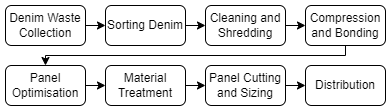
\includegraphics[width=0.5\textwidth]{figure/diagram.png}
\caption{Production Process of Acoustic Panels from Recycled Denim}
\label{fig:diagram}
\end{figure}
